%---------------------------------------------------------%
%______//------             GAC             ------\\______%
%______||------         Chapitre 7          ------||______%
%______\\------      Graphes de Cayley      ------//______%
%---------------------------------------------------------%

\chapter{Graphes de Cayley (groupes comme espaces métriques)}
\label{sec:graphes-de-Cayley}

  Soit $G$ un groupe, $S \subset G$ une partie symétrique ($s \in S \Rightarrow s^{-1} \in S$) et $1 \notin
  S$.

  \begin{defi} \index{Graphe!de Cayley}
    Le \emph{graphe de Cayley}, noté $\Gamma(G, S)$ est le graphe dont l'ensemble des sommets est $G$ est
    l'ensemble des arêtes est $E = \{(x,y) | xy^{-1} \in S \iff \exists s \in S\ :\ y = xs\}$.

    Deux sommets sont \emph{voisins}, et on les notes $x \sim y$, si $y$ s'obtient à partir de $x$ par
    multiplication par un élément de $S$.
  \end{defi}

  \begin{exs}
    \begin{enumerate}
    \item Soit $G = \Z/6\Z$ et $S = \{x, x^{-1}\}$, pour $x = 1$ et $x^{-1} = 5$.

    \item Soit $G = \Z/6\Z$ et $S = \{2, -2\}$.

    \item Soit $G = \Z/6\Z$ et $S = \{3 = -3\}$.

    \item Soit $G = \Z/6\Z$ et $S = \{2, -2, 3 = -3\}$.

    \item Soit $G = \Z$ et $S = \{1, -1\}$.

    \item Soit $G = \Z^2$ et $S = \{(\pm 1, 0), (0, \pm 1)\}$.

    \item Soit $G = \F_2 = \F(a,b)$ le groupe libre avec 2 générateurs et soit $S = \{a^{\pm 1}, b^{\pm 1}\}$.
    \end{enumerate}
  \end{exs}

  \begin{propri}
    \begin{enumerate}
    \item $\Gamma(G,S)$ est $k$-régulier, où $k = |S|$ (c'est-à-dire tout sommet a $k$ voisins).
    \item $\Gamma(G,S)$ et connexe $\iff$ $S$ engendre $G$.
    \end{enumerate}
  \end{propri}

  \begin{defi} \index{Arbre}
    Un \emph{arbre} un graphe connexe sans chemins fermés.
  \end{defi}

  \begin{prop}
    Soit $G$ un groupe et $S \subseteq G$ un ensemble. Alors $G cong \F(S)$ (le groupe libre sur $S$) si et
    seulement si $\Gamma(G, S)$ est un arbre.
  \end{prop}


  \begin{defi}
    Soient $\Gamma_1 = (V_1, E_1)$ et $\Gamma_2 = (V_2, E_2)$ deux graphes. Un \emph{morphisme de graphe}
    \index{Morphisme!de graphe} est une application $\phi: \Gamma_1 \to \Gamma_2$, $\phi \big|_V : V_1 \to
    V_2$, $\phi \big|_E : E_1 \to E_2$ telle que $(\phi(v), \phi(v')) \in E_2 \iff (v, v') \in E_1$.

    Si $\phi$ est bijective et $\Gamma_1 = \Gamma_2$, $\phi$ s'appelle un \emph{automorphisme de graphe}.
    \index{Automorphisme!de graphe}

    L'ensemble de tous les automorphisme de $\Gamma$, noté $Aut(\Gamma)$ forme un groupe.
  \end{defi}


  \begin{theo}
    Soit $G$ un groupe dénombrable. Alors il y a un graphe connexe $X$ tel que $G \cong Aut(X)$.
  \end{theo}

  \begin{preuve}
    Soit $S = \{s_1, s_2, \ldots \}$ un ensemble dénombrable de générateurs, c'est-à-dire que $G = \langle S
    \rangle$. Soit $X_0 = \Gamma(G,S)$ le graphe de Cayley de $G$ par rapport à $S$. Il faut se convaincre que
    $G \not\cong Aut(X_0)$.

    Pour chaque $i \geq 1$, soit $T_i$ un arbre fini (qui correspond à $s_i$)
    \begin{center}
      Figure de $T_i$ ici.
    \end{center}
    Si $i \neq j$, on a que $T_i \not\cong T_j$, car on n'a pas le même nombre de sommets dans $T_i$ et
    $T_j$. On doit montrer que $Aut(T_i) = \{id\}$ (exercice). 

    Dans le graphe de Cayley $X_0$, on remplace chaque arête $s_i$ par $T_i$, par exemple
    \begin{center}
      Dessiner exemple ici
    \end{center}
    et on obtient un graphe $X$. On a ainsi une expansion de $X_0$ vers $X$ ainsi qu'une contraction de $X$
    vers $X_0$ (en remplaçant $T_i$ par $s_i$). On observe que chaque automorphisme $\phi: X \to X$ induit un
    automorphisme $\phi_0: X_0 \to X_0$. 
    \begin{enumerate}
    \item Si $\gamma \in Aut(X)$ fixe $x \in V(X)$ ($\gamma(x) = x$), alors $\gamma = id_X$. En effet, si $x
      \in V(X) \setminus V(X_0)$ et $\gamma(x) = x$, alors $x \in V(T_i) \setminus \{a_i, b_i\}$. Ainsi
      $\gamma(T_i) = T_i$. Supposons que $x \in V(X_0)$ et $\gamma(T_{x,j}) = T_{x,j}$ pour chaque $x \in
      T_{x,j}$. L'idée est que si on fixe un tel $x$, on est obligé de fixer l'arbre $T_{x,j}$ (car deux
      arbres différents ne sont pas isomorphes), ainsi on fixe tous les arbres, donc toutes les arêtes et
      ainsi on fixe $xs_i$ pour chaque $i$, et par le Lemme de Zorn (car c'est un arbre infini, donc on doit
      faire ce processus à l'infini), on fixe l'arbre. C'est-à-dire que $\gamma(X) = X$, donc $\gamma = id$.

    \item $Aut(X) \cong G$. Soit $\phi: G \to Aut(X)$, $g \mapsto \phi_g$ où $\phi_g : X \to X$ est une
      extension de $\phi_g^0: X_0 \to X_0$ et $\phi_g^0(v) = gv$ si $v \in V(X_0) = G$. Commençons par montrer
      que $\phi$ est injective. On a
      \begin{align*}
        \phi(g) = \phi(g') &\iff \phi_g(v) = \phi_{g'}(v)\\
        &\iff gv = g'v\\
        &\iff g = g'
      \end{align*}
      Montrons à présent que $\phi$ est surjective. Soit $\psi \in Aut(X)$ avec $\psi(v) = v'$ pour $v,v' \in
      X_0$, alors il existe $g \in G$ tel que $\phi_g(v) = v'$ (par exemple on prend $g = v'v^{-1}$). On a
      $\psi(v) = \phi_g(v)$, et ainsi $(\psi^{-1}\phi_g)(v) = v$ et par la première observation,
      $\psi^{-1}\phi_g = id$ et donc $\psi = \phi_g$. \qedhere
    \end{enumerate}
  \end{preuve}

  \begin{rem}
    Si on change l'ensemble $S$, les graphes de Cayley pour $G$ sont différents entre eux (c'est-à-dire qu'ils
    ne sont pas isomorphes, en général). Mais ils sont \emph{quasi-isométriques} \index{Graphe!quasi-isométrique}
  \end{rem}


  À présent, on supposera toujours que $S$ engendre $G$ (sinon le graphe n'est pas connexe, et on n'a pas des
  bonnes propriétés).

  \begin{defi} \index{Longueur d'un mot $g$}
    Soit $g \in G$. La \emph{longueur} des mots de $g$ est la distance de $g$ à $\epsilon$ dans $\Gamma(G,S)$.
      \[|g|_S := \min\{n \in \N\ |\ g = s_1\cdots s_n,\ s_i \in S\}.\]

    Pour $g \in G$, la \emph{distance} de $x$ a $y$ \index{distance entre deux mots} est celle dans
    $\Gamma(G,S)$, notée $d_S(x,y) = |x^{-1}y|_S$.
  \end{defi}

  \begin{obss}
    \begin{enumerate}
    \item $d_S: G \times G \to \N$ est une distance sur $G$, invariante par l'action à gauche de $G$, $d_S(gx,
      gy) = d_S(x,y)$.

    \item Cette distance dépend du choix d'un système de générateurs $S$. Mais on va voir qu'en regardant le
      groupe \og de loin\fg, plusieurs propriétés importantes ne dépendent pas de $S$ (Gromov, $\sim 1980$).
    \end{enumerate}
  \end{obss}

  \begin{ex}
    Considérons $G = \Z$ et $S = \{\pm 1\}$. Le graphe de Cayley est simplement une droite infinie à gauche et
    à droite. Si à présent on considère $S' = \{\pm 2, \pm 3\}$, le graphe de Cayley devient 
    \begin{center}
    
            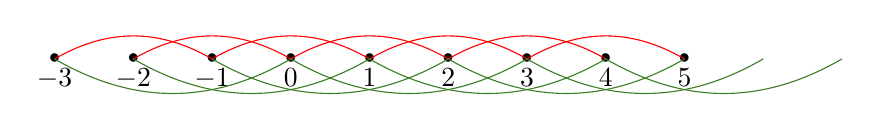
\begin{tikzpicture}
              \foreach \k in {-3,-2,...,5} { \draw (\k, 0) node[scale=0.8]{$\bullet$} node[below]{$\k$}; }
              \foreach \k in {-3, -2, ..., 3}{ \draw[color = red] (\k, 0) to[bend left] ({\k+2}, 0); }
              \foreach \k in {-3, -2, ..., 4}{ \draw[color = OliveGreen] (\k, 0) to[bend right] ({\k+3}, 0); }
            \end{tikzpicture}

          \end{center}
  \end{ex}



  \section{Quasi-isométries}
  \label{sec:quasi-isometries}

  
  Soient $(X, d)$, $(X', d')$ deux espaces métriques.

  \begin{defi}
    Une application $f: X \to X'$ est une \emph{quasi-isométrie} \index{Quasi-isométrie} s'il existe $g: X' \to
    X$ et des constante $\lambda >0$, $c \geq 0$ telles que
    \begin{enumerate}
    \item $d'(f(x), f(y)) \leq \lambda d(x,y) + c$ pour tout $x, y \in X$;
    \item $d(g(x'), g(y')) \leq \lambda d'(x', y') + c$ pour tout $x', y' \in X'$;
    \item $d(g(f(x)), x) \leq c$ pour tout $x \in X$;
    \item $d'(f'(g'(x')), x') \leq c$ pour tout $x' \in X'$.
    \end{enumerate}
    Les deux premières inégalités disent que $f, g$ sont Lipschitzienne à grande échelle. Les deux dernières
    disent que $f, g$ sont \emph{quasi-inverses} \index{Quasi-inverses} l'une de l'autre.
    On dit que $(X, d)$ et $(X', d')$ sont \emph{quasi-isométriques} \index{Espaces!quasi-isométriques} s'il
    existe une quasi-isométrie $f: X \to X'$.
  \end{defi}


  \begin{exs}
    \begin{enumerate}
    \item Soit $X = \R$ et $X' = \Z$. Considérons $f(x) = [x]$ (partie entière de $x$). Alors $f$ une
      quasi-isométrie (qi) avec $\lambda = c = 1$.

    \item Un espace borné est qi à un point (si on regarde l'espace de très très loin, il est réduit à un
      point).
    \item \textbf{Exercice:} Être qi est une relation d'équivalence parmi les espaces métriques.
    \end{enumerate}
  \end{exs}


  \begin{prop}
    Soient $S, T$ deux parties génératrices finies de $G$. Les espaces $\Gamma(G, S)$ et $\Gamma(G, T)$ sont qi.
  \end{prop}

  \begin{preuve}
    L'idée de la preuve est que chaque $s \in S$ est un mot dans $T$.
  \end{preuve}


  \begin{prop}
    Soit $G$ un groupe et $H \leq G$ un sous-groupe de $G$ d'indice fini ($|G:H| < \infty$). Alors $G$ et $H$
    sont qi.
  \end{prop}

  \begin{preuve}
    On démontrera ce résultat comme corollaire d'autres résultats plus généraux.
  \end{preuve}

  
  
  \section{Actions propres}
  \label{sec:actions-propres}

  \begin{defi}
    Soit $G$ un groupe agissant par homéomorphismes sur un espace topologique séparé $X$. L'action de $G$ sur
    $X$ est \emph{propre} \index{Action!propre} si pour tout $K, L \subset X$ parties compactes 
      \[\left| \{g \in G\ |\ gK \cap L \neq \varnothing \}\right| < \infty.\]
    Intuitivement, on ne peut pas avoir une infinité d'élément des copies de $K$ par l'action de $G$ qui
    intersecte $L$.
  \end{defi}

  \begin{prop}
    Supposons que $K = L = \{x\}$, on voit que dans une action propre, tout stabilisateur est fini.
      \[\mathrm{Stab}_G(x) = \{g \in G | gx = x\}.\]
  \end{prop}

  \begin{preuve}
    En fait on a que
    {
      \begin{align*}
        \{gx\} \cap \{x\} \neq \varnothing &\iff \{gx\} \cap \{x\} = \{x\}\\
        & \iff gx = x
      \end{align*}}
    et donc c'est assez clair.
  \end{preuve}


  \begin{exs}
    \begin{enumerate}
    \item Toute action d'un groupe fini est propre.
    \item Si $G$ agit sur $X$ avec $X$ compact, l'action est propre si et seulement si $G$ est fini. Il suffit
      de prendre $K = L = X$.
    \item L'action de $\Z^n$ sur $\R^n$ par translations est propre. 

      \textbf{Preuve:} Soient $K, L \subset \R^n$ deux parties compactes. Soit $v$ tel que $(v + K) \cap L
      \neq \varnothing$ (ici on travaille avec des vecteurs, donc la translation est représentée par le
      "+"). si et seulement s'il existe $k \in K$ et $l\in L$ tels que $v + k = l$ ss'il existe $k \in K$ et
      $l \in L$ tels que $v = l-k$ si et seulement si $v \in L \setminus K$ ($L \setminus K = C$ est
      compact). Alors $v \in C \cap \Z^n$ est fini, ce qui conclut. \qed

    \item Si $X$ est discret, l'action de $G$ sur $X$ est propre si et seulement si tous les stabilisateurs
      sont finis.

      \textbf{Preuve:} Montrons que si tous les stabilisateurs sont finis, alors l'action de $G$ sur $X$ est
      propre. Si $K, L \subset X$ sont compacts, alors ils sont finis. On peut donc écrire $K = \{x_1, \ldots,
      x_m\}$ et $L = \{y_1, \ldots, y_n\}$. On a 
      {
        \begin{align*}
          gK \cap L \neq \varnothing & \iff \exists i,j \text{ tq } gx_i = y_j.
        \end{align*}
      }
      $\{g \in G | gx_i = y_j\}$ est fini; c'est une classe latérale de $\mathrm{Stab}_G(x_i)$. \qed

    \item \textbf{Exercice:} Soit $G$ un groupe agissant par multiplication à gauche sur $(X, d)$, on pose
      $\delta(Gx, Gy) = \inf\{d(gx, hy)\ |\ g, h \in G\}$. Montrer que $\delta$ est une distance sur l'espace
      des orbites $_G \diagdown ^X$ qui définit la topologie quotient.
    \end{enumerate}
  \end{exs}




  \begin{defi} \index{Espace!géodésique}
    Un espace métrique $(X, d)$ est \emph{géodésique} si pour tous $x, y \in X$ avec $\Delta = d(x,y)$, il
    existe $\gamma:[0, \Delta] \to X$ continue avec $\gamma(0) = x$, $\gamma(\Delta) = y$, et $d(\gamma(s),
    \gamma(t)) = |s-t|$ pour tous $s, t \in [0, \Delta]$. C'est équivalent à dire que deux points quelconques
    peuvent être joints par un chemin géodésique, c'est-à-dire une isométrie d'un intervalle de $\R$ dans $X$.
  \end{defi}

  \begin{exs}
    \begin{enumerate}
    \item $\R^n$ muni de la distance euclidienne est un espace géodésique.
    \item Tous les espaces normés sont géodésiques.

      \textbf{Preuve:} Soit $X$ un espace normé et soit $\Delta = \|x - y\|$. On prend $\gamma(t) = x +
      \frac{t}{\Delta}(y-x)$, et donc $\|\gamma(s) - \gamma(t)\| = \frac{|s-t|}{\Delta}\|y-x\| = |s-t|$. \qed

    \item $\R^2$ muni de la norme $\|(x_1, x_2)\| = |x_1| + |x_2|$ n'est pas uniquement géodésique,
      c'est-à-dire qu'il existe en général plusieurs chemins géodésiques entre deux points.

    \item Soit $\R^2 \setminus \{(0,0)\}$ muni de la métrique euclidienne n'est pas géodésique.

      
    \item Un graphe étant un espace métrique discret se plonge de manière canonique dans un espace géodésique,
      sa \emph{réalisation géométrique} \index{Réalisation géométrique} obtenue en remplaçant chaque arête par
      une copie isométrique de l'intervalle $[0,1]$.

      
    \item[5'.] Les graphes de Cayley $\Gamma(G, S)$, $\langle S \rangle = G$ sont des espaces géodésiques.
    \end{enumerate}
  \end{exs}
  
 

  \section{Théorème fondamental de la théorie géométrique des groupes}
  \label{sec:thm-fond-theorie-geom-groupes}


  \begin{theo}[Efremovich (1953), \v{S}varc (1959), Milnor (1968)] \index{Théorème!de Milnor-\v{S}varc}
    Soit $X$ un espace métrique géodésique, dont les boules fermées sont compactes. Soit $G$ un groupe
    agissant proprement par isométries sur $X$ avec $_G\diagdown^X$ compact. Alors $G$ est finiment engendré
    et quasi-isométrique à $X$.
  \end{theo}


  \begin{ex}
    Soit $X = \R^n$ et $G = \Z^n$. On a une action propre de $\Z^n$ sur $\R^n$ par translations. En effet
    $\R^n$ est un espace géodésique, les boules fermées sont compactes et les translations sont des
    isométries. Le quotient est compact et donc on a que $\Z^n$ est finiment engengré et quasi-isométrique à
    $\R^n$. 
  \end{ex}

  

  




%%% Local Variables:
%%% mode: latex
%%% TeX-master: "../GAC_cours.tex" 
%%% End: